\section{$\phi$-symmetry in the hit rates}
\label{sec:phisymmetry}

The inclusive hit rates as a function of the transverse distance from the beam pipe are presented split into $\phi$-sectors. Figure~\ref{fig:hitrates-vs-r-phi-data} shows the hit rates in Run 284285 and Figure~\ref{fig:hitrates-vs-r-phi-mc} shows the hit rates in Pythia minimum bias simulation. Some shape differences appear between data and simulation which are under discussion.

\begin{figure}
  \begin{center}
    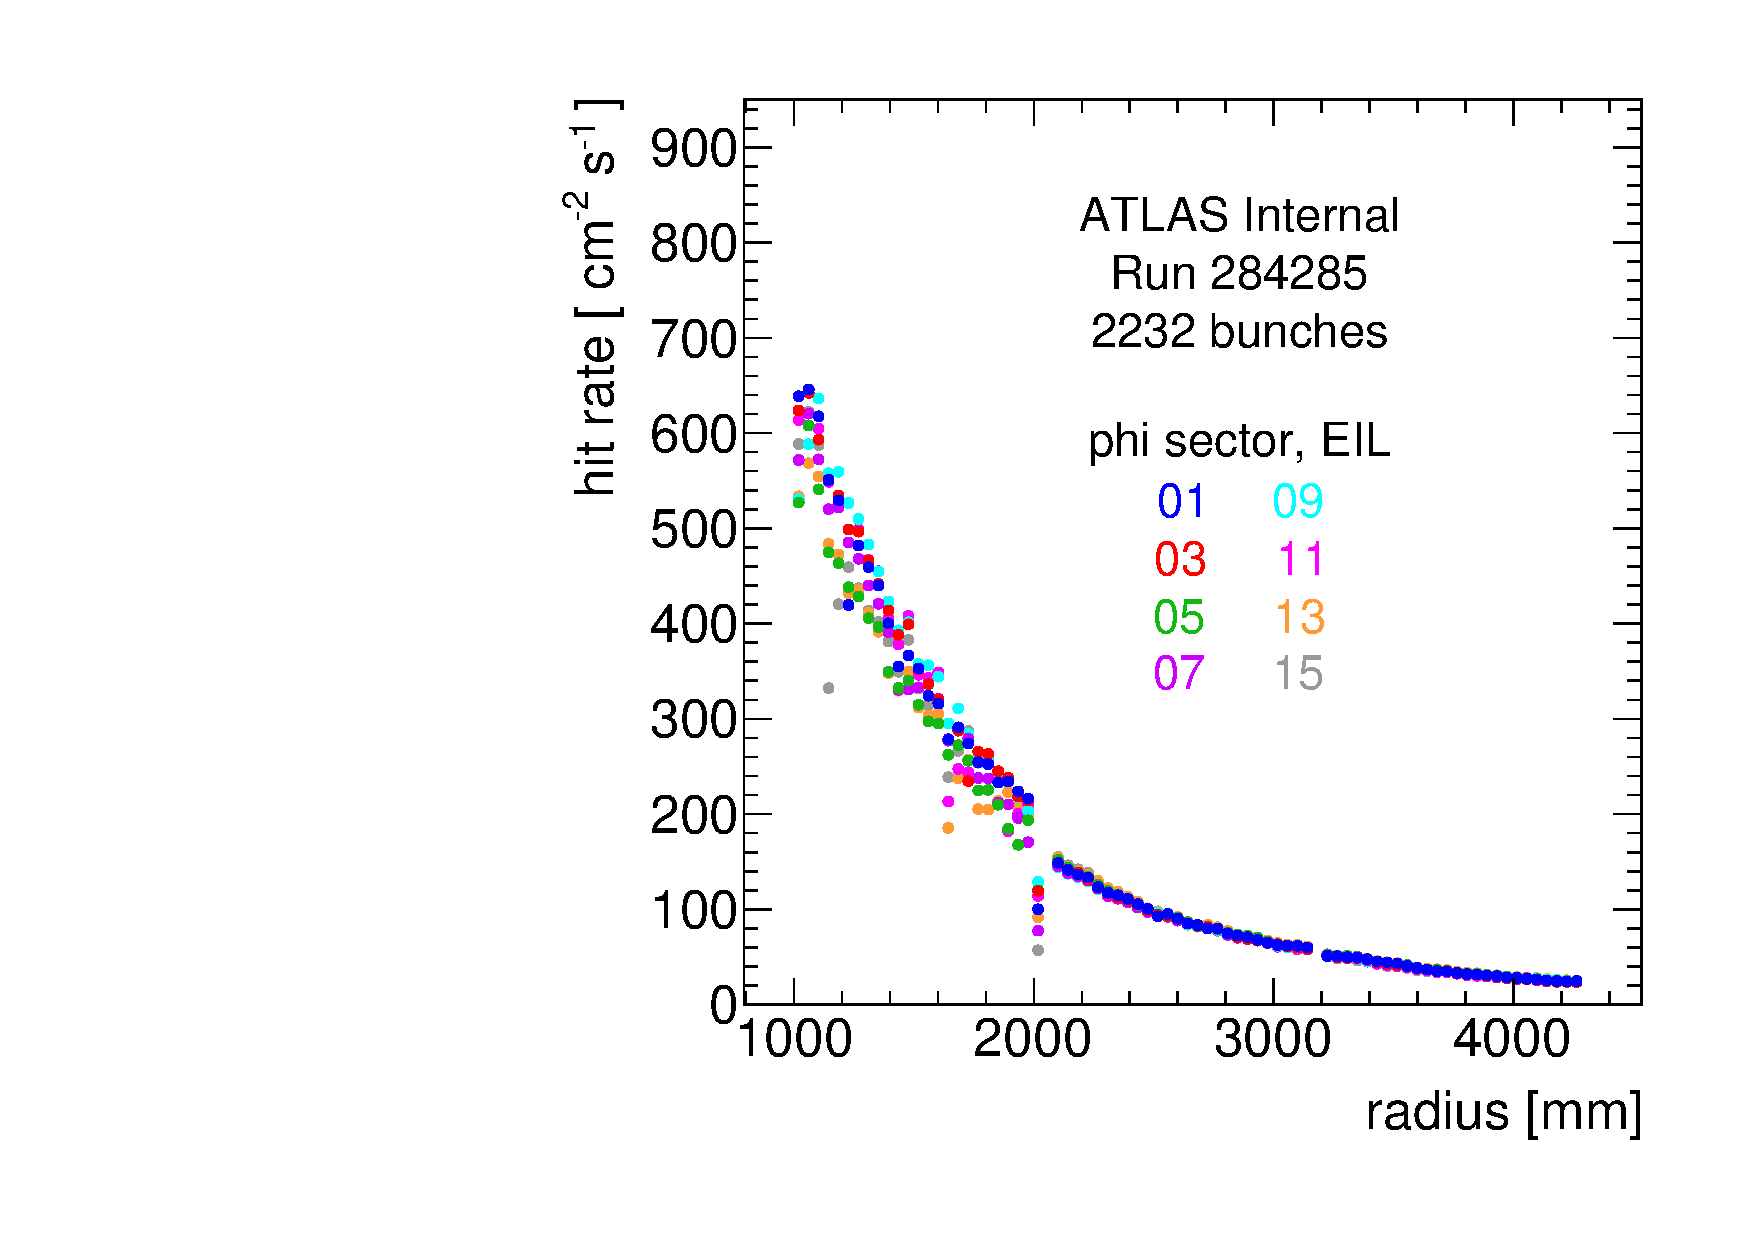
\includegraphics[width=0.45\textwidth]{./figures/rate_raw_vs_r_phi_EIL_00284285.pdf}
    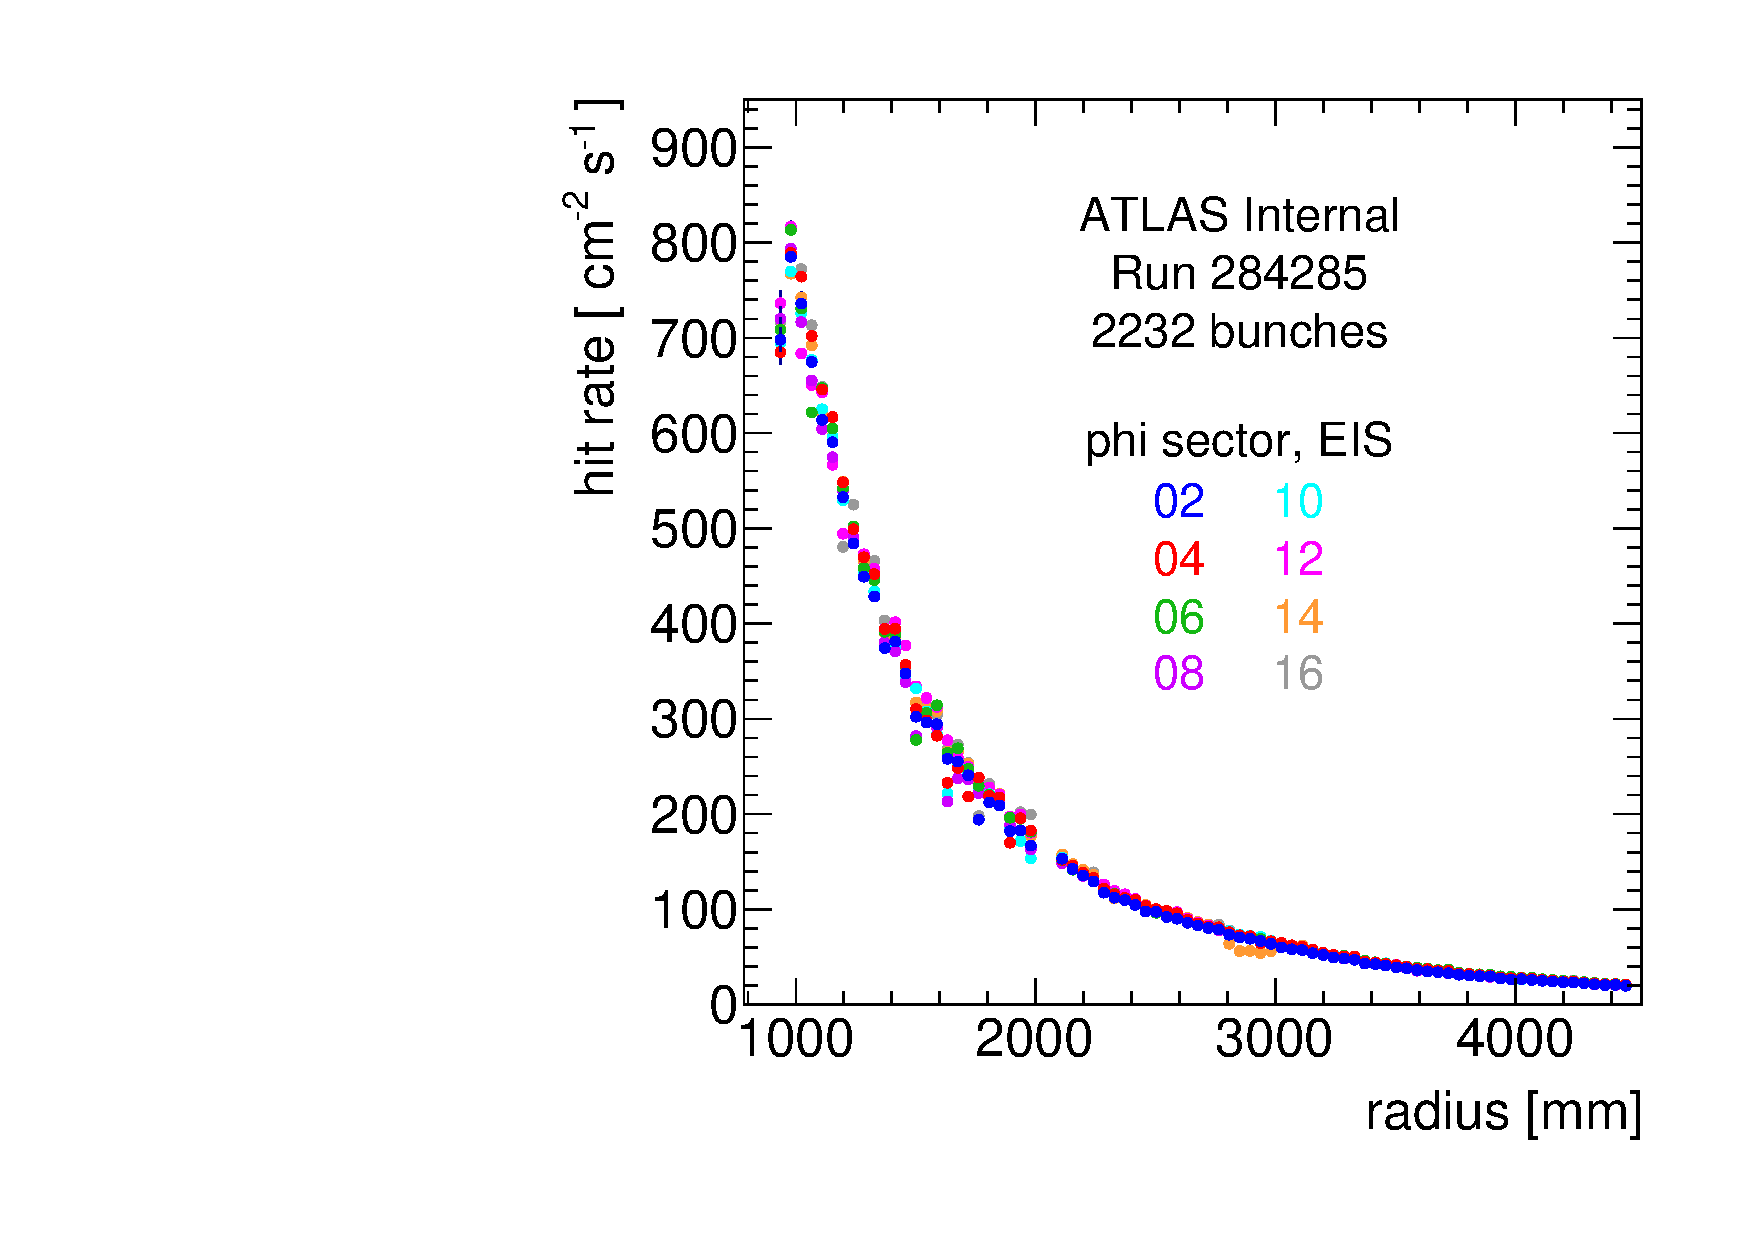
\includegraphics[width=0.45\textwidth]{./figures/rate_raw_vs_r_phi_EIS_00284285.pdf}
    \caption{Inclusive hit rate as a function of the transverse distance from the beam pipe in the small wheel split into $\phi$-sectors, for large (left) and small (right) sectors, in Run 284285.}
    \label{fig:hitrates-vs-r-phi-data}
  \end{center}
\end{figure}

\begin{figure}
  \begin{center}
    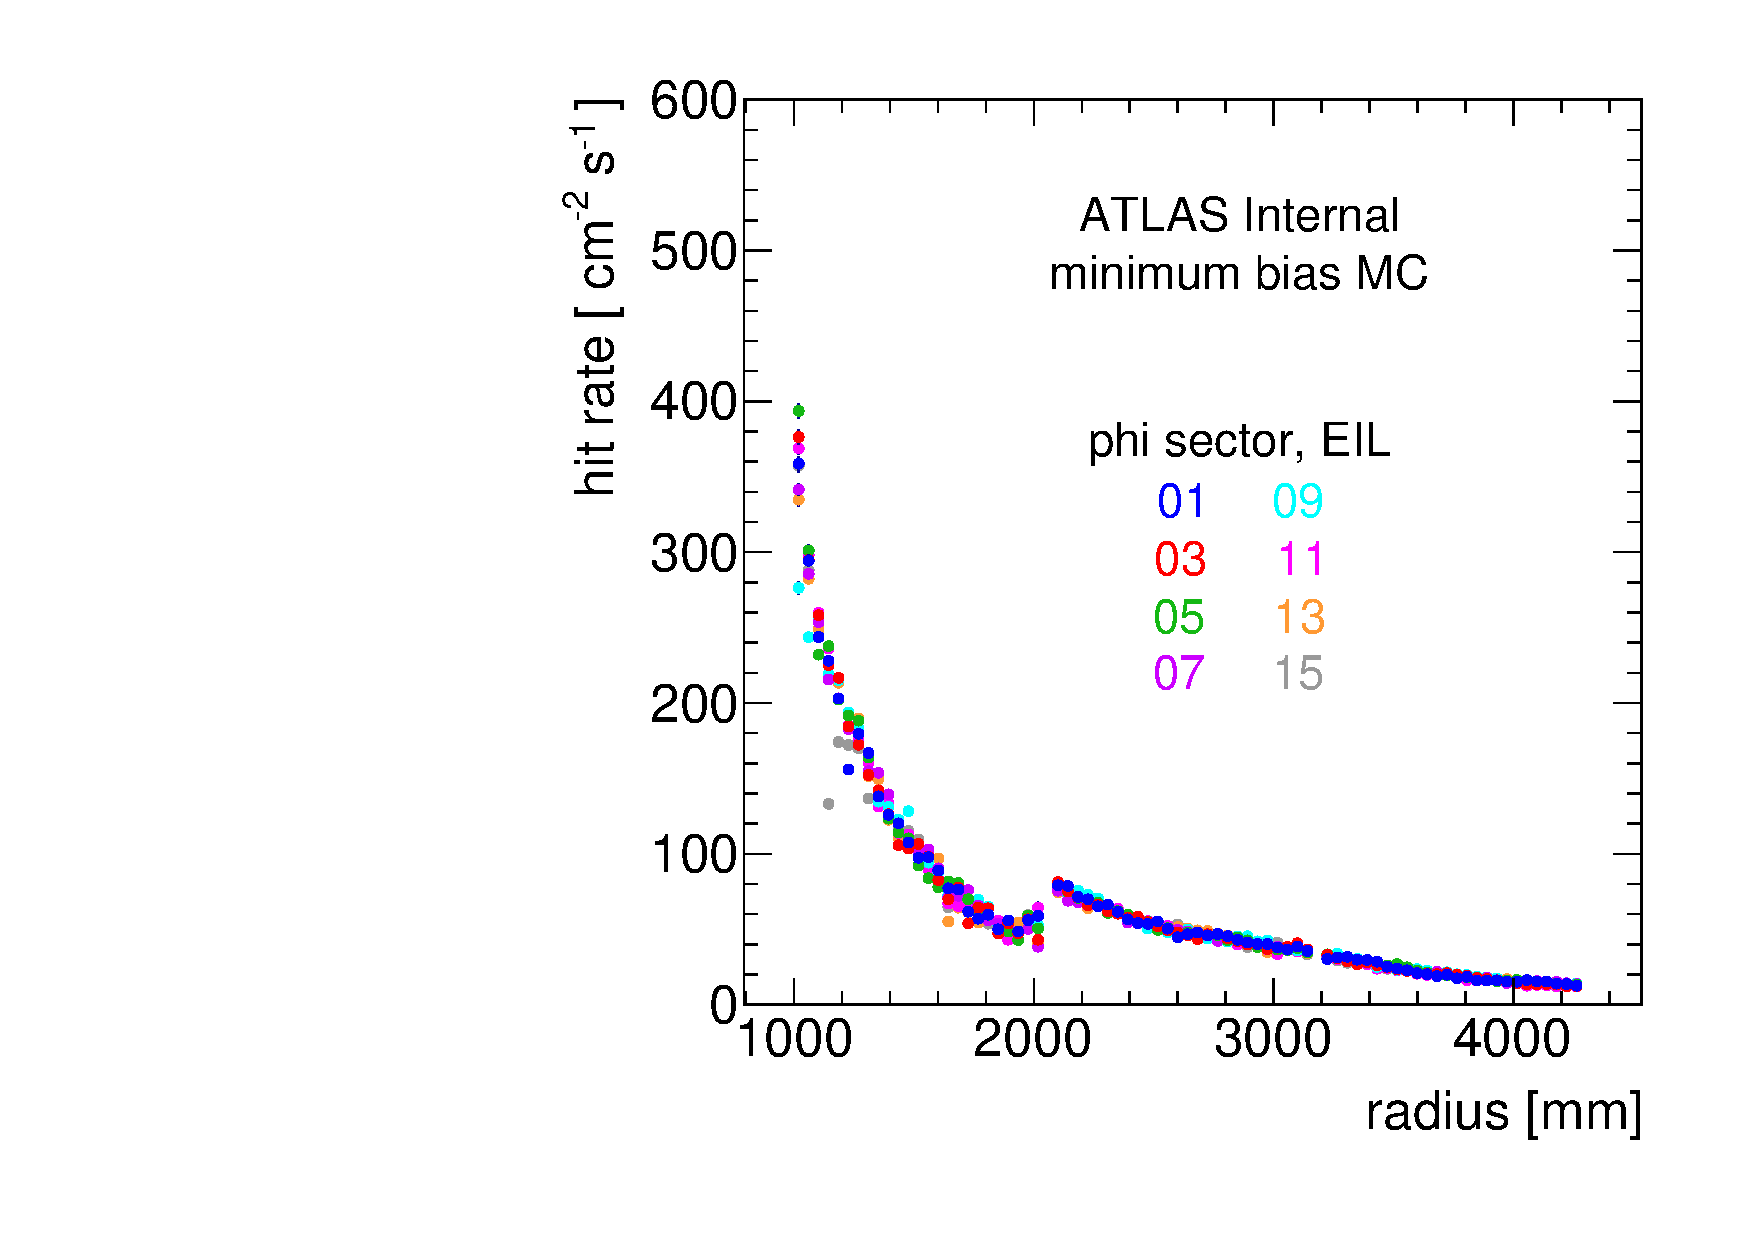
\includegraphics[width=0.45\textwidth]{./figures/rate_raw_vs_r_phi_EIL_00119994.pdf}
    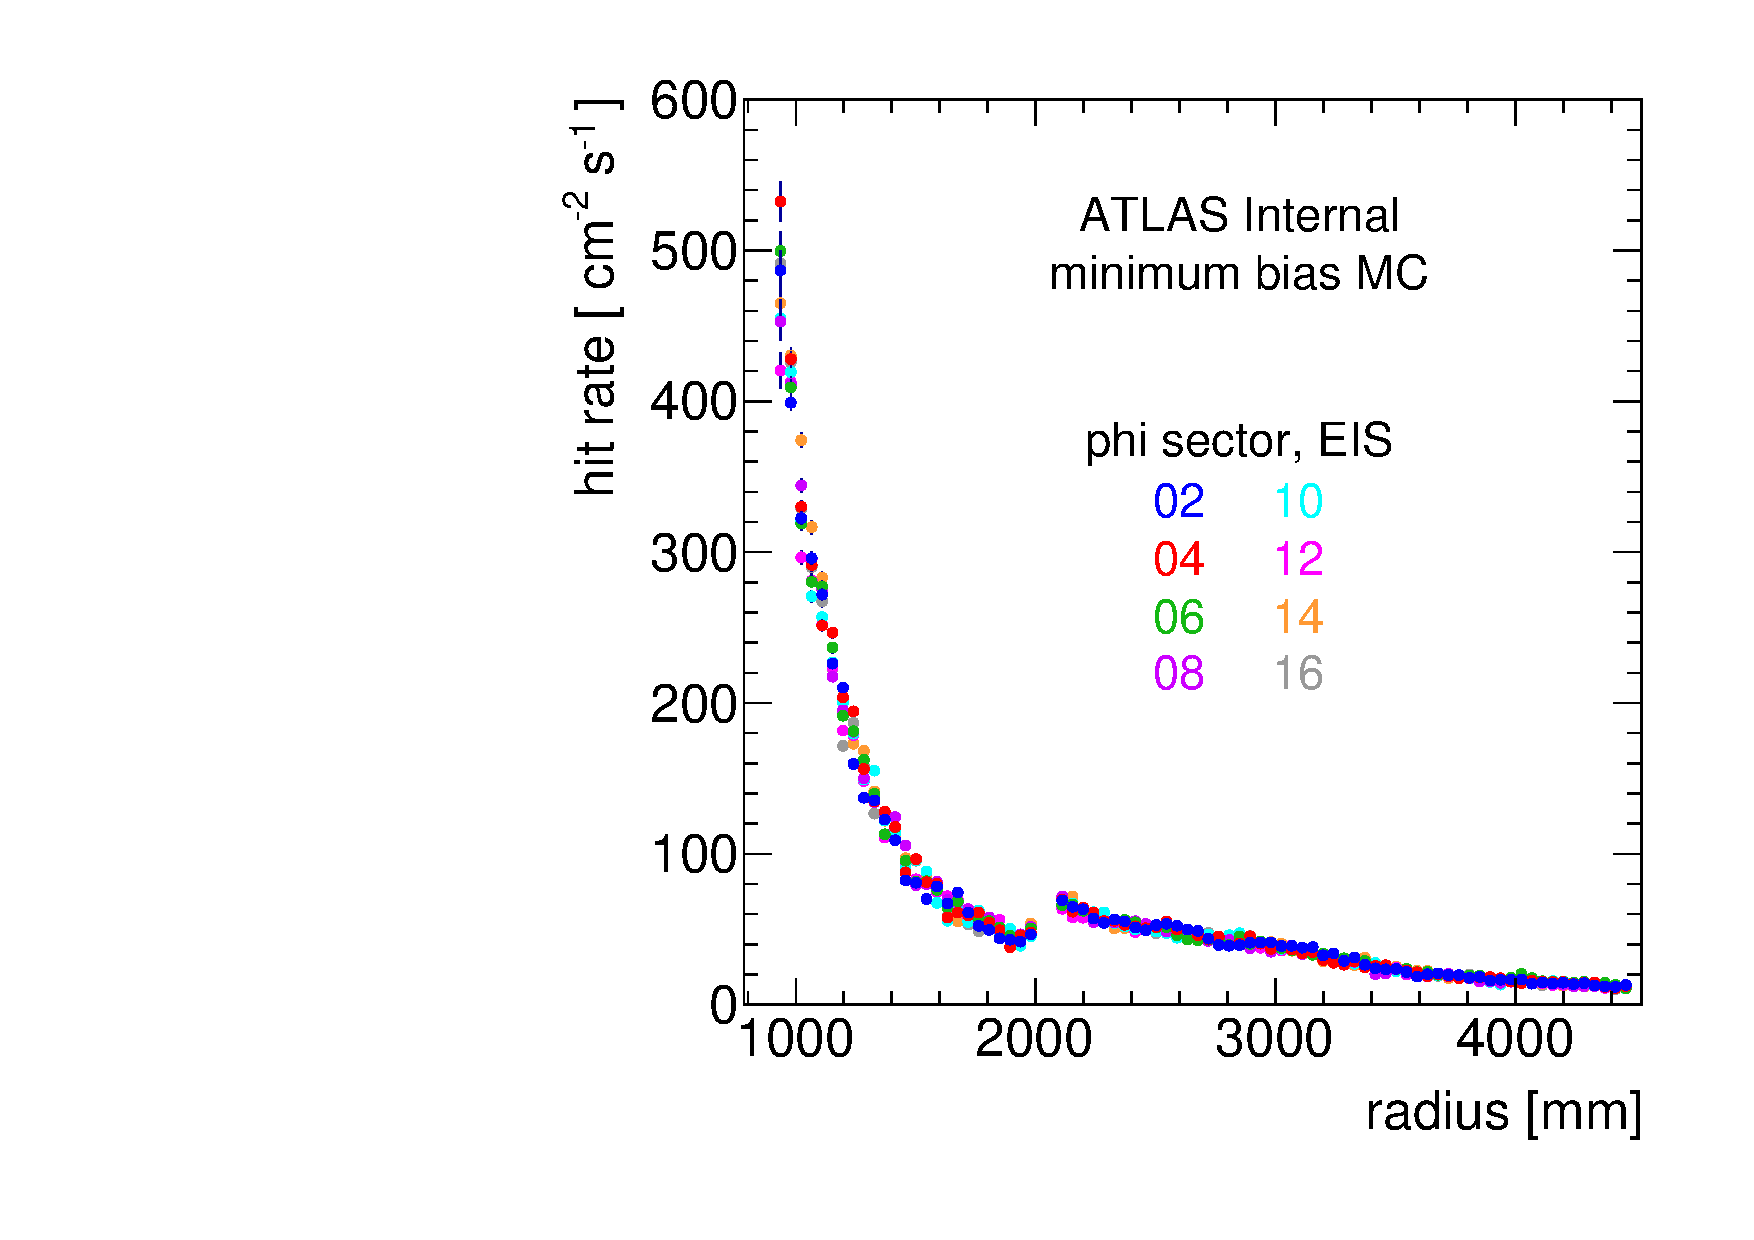
\includegraphics[width=0.45\textwidth]{./figures/rate_raw_vs_r_phi_EIS_00119994.pdf}
    \caption{Inclusive hit rate as a function of the transverse distance from the beam pipe in the small wheel split into $\phi$-sectors, for large (left) and small (right) sectors, in Pythia minimum bias simulation.}
    \label{fig:hitrates-vs-r-phi-mc}
  \end{center}
\end{figure}


